\newpage


\section{Стягивание ребер в $k$-связном графе}

\subsection{Минимальные по стягиванию 4-связные графы: лемма о треугольнике.}

\begin{df*}[Минимальный по стягиванию граф]
	Назовем $k$-связный граф $G$ \textbf{минимальным по стягиванию}, если для любого ребра $e \in E(G)$ граф $G \cdot e$ не является  $k$-связным. Где  $\cdot$ это операция стягивания ребра.
\end{df*}

\begin{df*}[Фрагмент и граница]
	Пусть $S \in \R_k(G)$, а $H$ ~-- компонента связности графа $G - S$, будем называть $H$ \textbf{фрагментом}.
	Множество $S$ будем называть \textbf{границей} фрагмента $H$ и обозначать $\Bound(H)$.
\end{df*}

\begin{remrk*}
	Фрагменты это внутренности частей разбиения одним разделяющим множеством.

	Также, если $H$ ~-- фрагмент, то $\Bound(H) = \N_G(H)$.
\end{remrk*}

\begin{customlm}{4.0} \label{lemma:4_0}
	Пусть $H$ ~-- фрагмент графа $G, \; T \in \R_k(G), T \cap H \neq \varnothing$, причем множество  $T$ независимо с границей фрагмента $H$. Тогда $T \not \supset H$ и существует фрагмент $H' \subsetneq H$ с границей $T$.
\end{customlm}

\begin{proof}
	Обозначим $S = \Bound(H), A = S \cup H \implies A \in \Part(S)$.

\begin{figure}[ht]
    \centering
	\incfig[0.3]{lemma_4_0}
	\caption{Рисунок к Лемме \ref{lemma:4_0}.}
    \label{fig:lemma_4_0}
\end{figure}

	Т.к. $T$ независимо с  $S \implies T \subset A \implies \exists A' \in \Part(T) \colon A' \subset A \implies \Int(A') \subset H$.

	А значит и $T \not \supset H$, ведь  $T \not \supset H' \subset H$.
\end{proof}

В следующих леммах и теореме речь пойдет о минимальных по стягиванию 4-связных графах.
Т.е. $v(G) > 5$ и для каждого ребра  $ab \in E(G)$ существует $T_{ab} \in \R_4(G) \colon a, b \in T_{ab}$.

\begin{customlm}{4.1} \label{lemma:4_1}
	Пусть $G$ ~-- минимальный по стягиванию 4-связный граф, множество $S \in \R_4(G)$ содержит $a$ и смежную с ней вершину, $H$ ~-- фрагмент с границей $S$. Тогда $a$ входит в треугольник $axx'$, где $x \in H, \deg_G(x) = 4$.
\end{customlm}

\begin{proof}
	Индукция по $|H|$.

	\begin{figure}[ht]
    \centering
	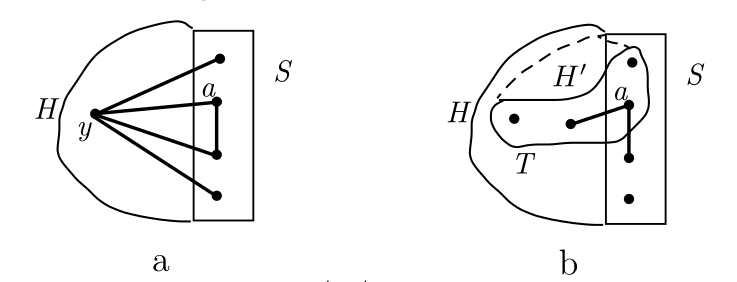
\includegraphics[width=0.4\columnwidth]{figures/lemma_4_1.png}
	\caption{Рисунок к Лемме \ref{lemma:4_1}.}
    \label{fig:lemma_4_1}
	\end{figure}

	База $H = \{y\}$, Рис. \eqref{fig:lemma_4_1}(a). В этом случае $\deg_G(y) = 4 \implies y$ смежна только с вершинами  $S$.

	Тогда нам подойдут  $x = y, x'$ ~-- смежная с  $a$ вершина  $S$.

	Считаем $|H| \geqslant 2$.

	Пусть  $A, A' \in \Part(S), \Int(A) = H$. Рассмотрим два случая:

	\begin{itemize}
		\item 1.: $\Let $Существует независимое с $S$ множество $T \in \R_4(G)$, что  $T \cap H \neq \varnothing$ и  $T$ содержит $a$ и смежную с ней вершину.

			Тогда $T \subset A$ и по Лемме \ref{lemma:4_0} существует фрагмент $H' \subsetneq H$ с границей $T$, см Рис. \eqref{fig:lemma_4_1}(b), по индукционному предположению существует искомый треугольник  $x \in H' \subset H$.

		\item 2.: $\Let $ Любое множество  $T \in \R_4(G) \colon T \cap H \neq \varnothing$ и  $T$ содержит  $a$ и смежную с ней вершину, зависимо с $S$.

			Существует вершина $b \in H$, смежная с  $a$(т.к. $a \in S$), рассмотрим множество $T_{ab}$. В нашем случае значит $T_{ab}$ и  $S$ зависимы.

			Пусть $T_{ab} = \{a, b, c_1, c_2\}$. Т.к. $T_{ab}$ пересекает внутренности всех частей  $\Part(S)$ \todo{почему?}, можно считать, что  $c_2 \in \Int(A')$.

			Рассмотрим еще два случая:

		\item 2.1: $\Let c_1 \not \in \Int(A)$. А значит $T_{ab} \cap \Int(A) = \{b\}$, т.к.  $|\Int(A)| = |H| \geqslant 2 \implies $ существует часть  $B \in \Part(\{S, T_{ab}\}) \colon B \subset A, \Int(B) \neq \varnothing$.
			Тогда  $|\Bound(B)| \geqslant 4$, пусть  $B = A \cap F$, где  $F \in \Part(T_{ab})$, см. Рис. \ref{fig:lemma_4_1.2}(a).

			Но $\Bound(B)$ состоит из вершины  $b$ и вершин множества  $S$, лежащих в  $F$.
			А их не более трёх(ведь $S$ пересекает внутренность отличной от  $F$ части  $\Part(T_{ab})$).
			А значит $\Bound(B) = 4$.
			Таким образом,  $a, b \in \Bound(B), \Bound(B) \in \R_4(G)$, множества  $\Bound(B)$ и  $S$ независимы, противоречие с предположением.

	\begin{figure}[ht]
    \centering
	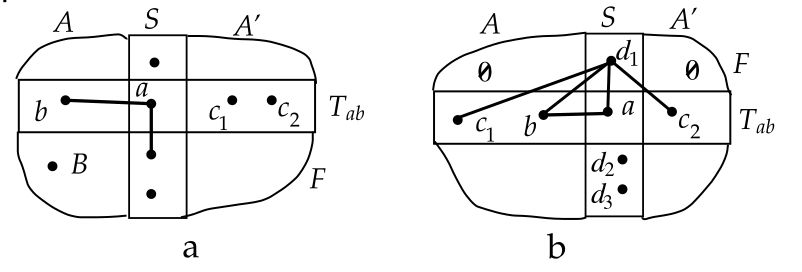
\includegraphics[width=0.5\columnwidth]{figures/lemma_4_1.2.png}
	\caption{Рисунок к Лемме \ref{lemma:4_1}.}
    \label{fig:lemma_4_1.2}
	\end{figure}

\item 2.2: $\Let c_1 \in \Int(A)$. Рисунок \ref{fig:lemma_4_1.2}(b) Тогда $T_{ab}\setminus A = \{c_2\}$. Т.к. $T_{ab}$ должно пересекать внутренность всех частей $\Part(S)$, то их только две: $A$ и $A'$.

	Пусть $S = \{a, d_1, d_2, d_3\}$. Тогда $S \cap T_{ab} = \{a\}$ и множество $T_{ab}$ разделяет $S \setminus T_{ab} = \{d_1, d_2, d_3\}$. Следовательно, $\exists F \in \Part(T_{ab}) \colon |F \cap \{d_1, d_2, d_3\}| = 1$.

	Б.о.о. $F \cap \{d_1, d_2, d_3\} = \{d_1\}$, тогда $B = A \cap F \in \Part(\{S, T_{ab}\})$, причем $\Bound(B) = \{a, b, c_1, d_1\}$.

	Если  $\Int(B) \neq \varnothing$, то это противоречит нашему предположению.
	Тогда  считаем $\Int(B) = \varnothing$.

	Пусть  $B' = F \cap A'$, тогда $\Bound(B') = \{a, c_2, d_1\} \implies \Int(B') = \varnothing \implies \Int(F) = S \cap \Int(F) = \{d_1\} \implies \deg_G(d_1) = 4, N_G(d_1) = T_{ab} = \{a, b, c_1, c_2\}$. Получили практически то, что хотели, только $d_1 \in S$, а хотим вершину из $\Int(A)$.

	\end{itemize}


\begin{customclaim}{4.1} \label{claim:4_1}
	Пусть множество $S \in \R_4(G)$ содержит $a$ и смежную с ней вершину, $H$ ~-- фрагмент с границей $S$. Тогда $a$ входит в треугольник $azz'$, где одна из вершин $z$ и $z'$ лежит в $H$.
\end{customclaim}

\begin{proof}
	Ослабление Леммы \ref{lemma:4_1}.
	В случаях 1 и 2.1 мы осуществили спуск к меньшим фрагментам. Продолжая этот спуск мы либо придем к тривиальному случаю из одной вершины, либо к случаю 2.2, в котором показали существование треугольника $abd_1$, мы просто не показали что $\deg_G(b) = 4$.
\end{proof}

Продолжим наш случай 2.2:

Применим Утверждение \ref{claim:4_1} к множеству $S$, вершине  $d_1$ и фрагменту $\Int(A')$.

Т.к. в  $\Int(A')$ ровно одна вершина из $\N_G(d_1)$ ~-- $c_1$ и она не может быть смежна с $b, c_1$, т.к. они не лежат в $A'$, то значит вершины  $a$ и  $c_2$ смежны. Рисунок \eqref{fig:lemma_4_1.3}(a).

	\begin{figure}[ht]
    \centering
	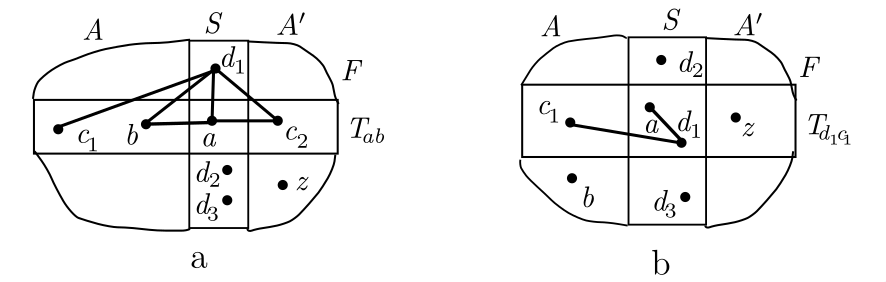
\includegraphics[width=0.5\columnwidth]{figures/lemma_4_1.3.png}
	\caption{Рисунок к Лемме \ref{lemma:4_1}, случаю 2.2.}
    \label{fig:lemma_4_1.3}
	\end{figure}

	Множество $T_{d_1c_1}$ должно быть зависимо с $T_{ab} = \Bound(F)$, т.к. $T_{d_1c_1} \supset \Int(F) = \{d_1\}$.

	Следовательно, $T_{d_1c_1}$ разделяет $T_{ab} \setminus T_{d_1c_1} \subset \{a, b, c_2\}$, а поскольку $a$ смежна с $b$ и $c_2$, то $a \in T_{d_1 c_1}$, а значит $T_{d_1c_1}$ зависимо с $S$, по предположению 2.

	Таким образом,  $T_{d_1 c_1} = \{d_1, c_1, a, z\}$, где $z \in \Int(A')$.

	Множество  $T_{d_1c_1}$ должно разделять $S \setminus T_{d_1c_1} = \{d_2, d_3\}$, поэтому $|\Part(T_{d_1c_1})| = 2$ и $T_{d_1c_1}$ делит $A$ на две части с границами $\{c_1, a, d_1, d_2\}$ и $\{c_1, a, d_1, d_3\}$, см. Рис. \eqref{fig:lemma_4_1.3}(b).

	Одна из этих частей содержит $b$ и поэтому не пуста, а её граница содержит $a$ и смежную с ней вершину $d_1$, а также лежит в $A$ и независима с $S$. Противоречию предположению 2.

\end{proof}

\subsection{Минимальный по стягиванию 4-связный граф 4-регулярен, каждое ребро входит в треугольник.}

\begin{customlm}{4.2}[N. Martinov, 1990] \label{lemma:4_2}
	Минимальный по стягиванию 4-связный граф является 4-регулярным.
\end{customlm}

\begin{proof}
	Т.к. граф является 4-связным, то степень любой вершины $\geqslant 4$, а значит утверждение верно для  $G \colon v(G) = 5$, далее считаем  $v(G) > 5$.

	Пусть $v \in V(G) \colon \deg_G(v) > 4$.

	По Лемме \ref{lemma:4_1} существует вершина $u \in \N_G(v) \colon \deg_G(u) = 4$ и  $u_1 \in \N_G(u) \colon \deg_G(u_1) = 4$.

	Рассмотрим множество $T_{u u_1}$, пусть $A_1, A_1' \in \Part(T_{uu_1})$, тогда по Лемме \ref{lemma:4_1} существуют вершины $u_2, u_3 \in \N_G(u)$, где $u_2 \in \Int(A_1), u_3 \in \Int(A_1') \colon \deg_G(u_2) = \deg_G(u_3) = 4$. Смотреть Рис. \eqref{fig:lemma_4_2}(a).

	Значит, $u_2$ и $u_3$ не смежны.

	\begin{figure}[ht]
    \centering
	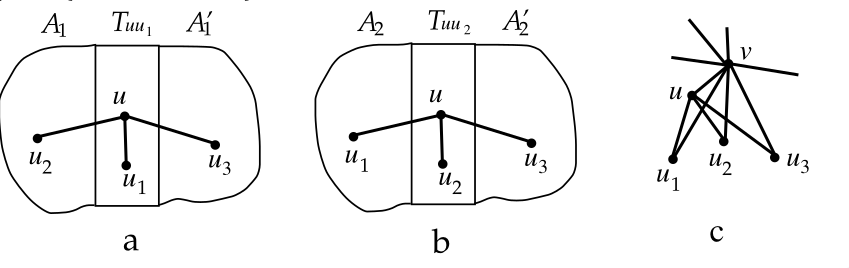
\includegraphics[width=0.6\columnwidth]{figures/lemma_4_2.png}
	\caption{Рисунок к Лемме \ref{lemma:4_2}.}
    \label{fig:lemma_4_2}
	\end{figure}

	Таким образом, $\N_G(u) = \{v, u_1, u_2, u_3\}$.

	Теперь рассмотрим $T_{uu_2}$, пусть $A_2, A_2' \in \Part(T_{uu_2})$, по Лемме \ref{lemma:4_1} в $\N_G(u)$ сущестуют вершины степени 4, одна из которых лежит в  $\Int(A_2)$, другая в $\Int(A_2')$.

	Это могут быть только вершины $u_1$ и $u_3$, значит они не смежны, смотреть Рис. \eqref{fig:lemma_4_2}(b).

	Аналогично $u_1, u_2$ не смежны.

	Теперь заметим, что по Лемме \ref{lemma:4_1} каждая из вершин $u_1, u_2, u_3$ должна входить в треугольник вместе с вершиной $u$, а следовательно все эти три вершины смежны с  $v$, ведь $\N_G(u) = \{v, u_1, u_2, u_3\}$.

	Таким образом, любая вершина $u \in \N_G(v)$ степени 4 имеет трёх попарно несмежных соседей степени 4, лежащих в  $\N_G(v)$, смотреть Рис. \ref{fig:lemma_4_2}(c).

	Тогда все вершины степени 4 смежные с $v$ образуют отдельную компоненту связности, а значит  $v$ не смежна с вершинами степени $> 4$(ведь была бы точкой сочленения, а граф 4-связный). 

	Тогда вершина  $v$ входит в любое множество из $\R_4(G)$, следовательно, граф $G - v$ является минимальным по стягиванию трёхсвязным графом.
	Как мы знаем, такой граф это $K_4$.
	Тогда  $G$ ~-- 4-регулярный граф на 5 вершинах, противоречие.

\end{proof}

\begin{customthm}{4.1}[N.Martinov, 1990] \label{theorem:4_1}
	Для 4-связного графа $G$ следующие два утверждения равносильны:

	\begin{enumerate}
		\item Граф $G$ ~-- минимальный по стягиванию
		\item Степень каждой вершины графа $G$ равна 4, каждое ребро входит в треугольник
	\end{enumerate}

\end{customthm}

\begin{proof}
	$2 \implies 1$: Если ребро $ab$ входит в треугольник  $abc$ и  $\deg_G(c) = 4$, то в графе  $G \cdot ab$ окрестность вершины  $c$ будет трёхвершинным множеством, поэтому граф  $G \cdot ab$ не 4 связен.

	$1 \implies 2$: По Лемме \ref{lemma:4_2} граф  $G$ является 4-регулярным.

	Найдем треугольник с ребром $uv \in E(G)$. 
	Рассмотрим разделяющее множество $T_{uv}$, пусть $A_1, A_2 \in \Part(T_{uv})$, по Лемме \ref{lemma:4_1} существуют треугольники $u u_1 u_1'$ и $u u_2 u_2'$, где $u_1 \in \Int(A_1), u_2 \in \Int(A_2)$.

	Если хотя бы одна из вершин $u_1', u_2'$ это $v$, то мы нашли искомый треугольник.

	Если  $u_1' \neq v, \; u_2' \neq v$, то т.к. $\deg_G(u) = 4 \implies u_1' = u_2' \in T_{uv}$. Обозначим эту вершину $u'$. Смотреть Рис. \eqref{fig:theorem_4_1}(a).

	\begin{figure}[ht]
    \centering
	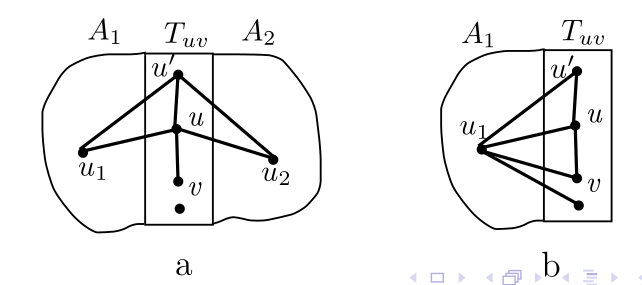
\includegraphics[width=0.5\columnwidth]{figures/theorem_4_1.png}
	\caption{Рисунок к Теореме \ref{theorem:4_1}.}
    \label{fig:theorem_4_1}
	\end{figure}

	Т.к. $\deg_G(u') = 4$ и  $u \in \N_G(u') \cap T_{uv}$, то одно из множеств $\Int(A_1), \Int(A_2)$ содержит единственную вершину из $\N_G(u')$, н.у.о. это  $\Int(A_1)$.
	Тогда $u_1$ ~-- единственная вершина из $\Int(A_1)$ смежная с $u$ и единственная вершина из  $\Int(A_1)$ смежная с $u'$.

	Если  $\Int(A_1) \neq \{u_1\}$, то трёхэлементное множество $(T_{uv} \setminus \{u, u'\}) \cup \{u_1\}$ отделяет $\Int(A_1) \setminus \{u_1\}$ от остальных вершин графа, что невозможно.

	Значит, $\Int(A_1) = \{u_1\}$, тогда $\N_G(u_1) = T_{uv}$, смотреть Рис. \eqref{fig:theorem_4_1}, в частности, в графе $G$ есть треугольник  $uvu_1$.

\end{proof}

\begin{customcrly}{4.1} \label{crly:4_1}
	В минимальном по стягиванию 4-связном графе $G$ все вершины имеют степень 4, а окрестность каждой вершины разбивается на две пары смежных вершин.
\end{customcrly}

\begin{proof}

	Предположим, что для вершины $a$ это не так.
	Пусть $\N_G(a) = \{b_1, b_2, b_3, b_4\}, \, A = \{a\} \cup \N_G(a)$.

	По Теореме \ref{theorem:4_1} ребро $ab_1$ входит в треугольник, б.о.о. это $ab_1b_2$.
	Тогда $b_1b_2 \in E(G)$, следовательно, $b_3b_4 \not \in E(G)$.

	Ребро $ab_3$ также входит в треугольник и это должен быть треугольник $ab_3b_1$ или $ab_3b_2$, н.у.о. это $ab_3b_1$.

	Тогда $b_1b_3 \in E(G)$, следовательно, $b_2b_4 \not \in E(G)$.
	Значит, ребро $ab_4$ входит в треугольник $ab_1b_4$, то есть $b_1b_4 \in E(G)$, см рис. \eqref{fig:crly_4_1}.

	\begin{figure}[ht]
    \centering
	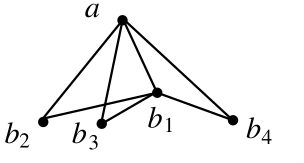
\includegraphics[width=0.25\columnwidth]{figures/crly_4_1.png}
	\caption{Рисунок к Следствию \ref{crly:4_1}.}
    \label{fig:crly_4_1}
	\end{figure}
	Но тогда $V(G) = A$, иначе  $\{b_2, b_3, b_4\}$ отделяет $\{a, b_1\}$ от $V(G) \setminus A$, что невозможно. Следовательно,  $G \simeq K_5$, а значит утверждение очевидно.


\end{proof}

\subsection{Классификация минимальных по стягиванию 4-связных графов.}

\begin{df*}[Степень графа]
	Для графа $G$ обозначим  $G^{k}$ ~-- $k$-ая \textbf{степень графа}. Это граф на тех же самых вершинах, где ребро $(u, v)$  проведено $\iff$ в исходном графе расстояние между  $u, v$ не больше  $k$. В частности, $G^{1} = G$.
\end{df*}

Тогда $C_n^{2}$ это квадрат цикла.

\begin{df*}[Рёберный граф]
	По графу  $G$ построим новый граф, у которого вершины это ребра исходного графа, а ребро соединяет две вершины, если соответствующие ребра в исходном графе имели общую вершину.
\end{df*}

Кубический граф это просто 3-регулярный.

\begin{figure}[ht]
    \centering
	\incfig[0.4]{cubic_edge_4_cyclic_connected}
    \caption{Образование треугольников в рёбёрном графе для кубического, 4-рёберно-циклически связного. Черным цветом обозначен исходный граф, бирюзовым ~-- рёберный граф.}
    \label{fig:cubic_edge_4_cyclic_connected}
\end{figure}

\subsection{Происхождение трёхсвязных графов от колеса.}

\todo[inline]{почему есть вершина степени 3? начало док-ва теоремы 3}

В док-ве теоремы 3, случай 1, когда берем множество $S= \{x, y, z\}$, то мы неявно говорим что  $z \neq t_1, z \neq t_2$. Это верно, т.к. $\{x, y, t_1\}$ и $\{x, y, t_2\}$ не являются разделяющими, это верно т.к. у $x$ должно быть хотя бы по одному ребру в каждую часть.
